\newpage
%%%%%%%%%%%%%%%%%%%%%%%%%%%%%%%%%%%%
\subsection{Towards a model of changes in organizing strategy}
\label{disc:study-discussion:changes-model}
%%%%%%%%%%%%%%%%%%%%%%%%%%%%%%%%%%%%



%%%%%%%%%%%%%%%%%%%%%%%%%%%%%%%
\subsection{MOVE PIM Strategies}
\label{discussion:strategies}
%%%%%%%%%%%%%%%%%%%%%%%%%%%%%%%

% This section offers a new conceptualization of PIM strategies.  Firstly, \textbf{Section~\ref{discussion:strategies-cross-tool}} develops a cross-tool model of PIM strategy, drawing from the cross-tool perspective developed in \textbf{Section~\ref{discussion:cross-tool}}.
Then, \textbf{Section~\ref{discussion:strategies-changes}} develops a model of changes in PIM strategy over time, extending the model proposed in~\citet{ob:97}.

%%%%%%%%%%%%%%%%%%%%%%%%%%%%%%%%%%%%%%%%%%%%%%%%%%%%%%
\subsection{Towards a new model of strategy changes}
\label{discussion:strategies-changes}
%%%%%%%%%%%%%%%%%%%%%%%%%%%%%%%%%%%%%%%%%%%%%%%%%%%%%%

PIM behaviour is not continuous, but may evolve over time as illustrated by the findings presented in \textbf{Chapter~\ref{chapter:main-study}}, and discussed in \textbf{Section~\ref{discussion:ongoing}}. Building on the observation of multiple strategies in \textbf{Chapter~\ref{chapter:exploratory_study}}, a new model of PIM strategy changes is proposed, as an initial step towards developing theory in this area.

When researchers talk about PIM strategies, they are describing \textit{average behaviour over the long-term}.  As discussed in the previous section, users may employ different strategies for different types of information (e.g. filing information related to some production tasks but not others).  In addition, the word ``strategy'' has the connotation that users devote time to selecting that strategy.  However in many cases, PIM strategies may not be pre-determined, but simply the amalgam of many spur-of-the-moment discrete events.

In addition, strategies may change over time.  They are not pre-determined, but may evolve.  Empirical data of real-life PIM strategies was presented in \textbf{Chapter~\ref{chapter:main-study}}.

%%%%%%%%%%%%%%%%%%%%%%%%%%%%%%%%%%%%%%%%%%%%%%%%%%%%%%%%%%%%%%%%%%%%%%%
% Build on Balter
% LINK TO THEORY DEV:BALTER: (towards improved model of changes in PIM strategies)
% (influencing factors are discussed). 
% Balter's study is based on an abstract classification, and the corners of his model represent overall extreme traits. Instead, what changes is the RATIO of information that is dealt with in a particular way
%%%%%%%%%%%%%%%%%%%%%%%%%%%%%%%%%%%%%%%%%%%%%%%%%%%%%%%%%%%%%%%%%%%%%%%
A model of changes in email organizing strategy was proposed in~\citep{ob:97}.  This can be criticised for focusing on major shifts in strategy between extreme user traits such as \textit{frequent filer} and \textit{spring cleaner}.  \textbf{Chapter~\ref{chapter:exploratory_study}} argued that such classifications were inaccurate as they portrayed abstract, extreme user traits.  % replace chapter with section

%%%%%%%%%%%%%%%%%%%%%%%%%%%%%%%%%%
% Multiple strategies revisited}
%%%%%%%%%%%%%%%%%%%%%%%%%%%%%%%%%%
% USE: relate to multiple strategies data 
% MS confirms ES: users again employ a range of strategies (EXPLORATORY CONFIRMATION). 
% /variegated/multi-faceted
% : one user - multiple strategies depending on type of information being managed
In this section, B�lter's model is extended to account for the change data collected in \textbf{Chapter~\ref{chapter:main-study}}. The observed changes were more incremental than those observed by B�lter.  They equated to \textit{shifts in the relative proportions of information managed with a particular strategy}. % Participants differed in the relative proportions of the low-level strategies employed. 


%%%%%%%%%%%%%%%%%%%%%%%%%%%%%%%%%%%%%%%%%%%%%%%%%%
% STUDY EXAMPLES: link changes with multiple strategies. 
%%%%%%%%%%%%%%%%%%%%%%%%%%%%%%%%%%%%%%%%%%%%%%%%%%
% In particular, it is suggested that small changes are made as demanded by new production activities and types of information.
The change data observed in the main study corresponds with the observation of \textit{multiple strategies} outlined in \textbf{Chapter~\ref{chapter:exploratory_study}}.  Multiple strategies were identified in the context of specific tools, as well as across multiple tools for most participants.  Here a focus is taken on changes within specific tools only.

Observed changes corresponded to small shifts in overall strategy.  Typically the change was highly targeted at how a specific type of information was managed.  Two participants made significant changes as follows:
\begin{itemize}

% worked on working information, few aspects, in certain tools (certain stuff?)
\item Participant F3 changed the way that he worked with certain type of active, working information -- moving it from ``My Documents'' to the ``Desktop'' and setting up a series of new sub-folders.

\item Participant M5 made two changes.  Firstly, he changed how he managed old information in both files and email -- moving all old project data under an ``Old'' folder in both collections.  Secondly, he changed the management of email for a specific production activity -- planning conferences to submit papers to.
% -- possibly driven by the demands of a new production activity taken up by the user in question.
% : one activity example. What about re-org of stuff into old? (actually managing working stuff in the same way)
\end{itemize}

%%%%%%%%%%%%%%%%%%%%%%%
% EXTEND THE MODEL
%%%%%%%%%%%%%%%%%%%%%%%
Based on the observations outlined above, B�lter's model of user strategy changes is extended to reflect the incremental strategy changes that were observed.  As in B�lter's work, a focus is taken on email, but the model can be also applied to other tool contexts\footnote{Note that different changes may happen simultaneously in different tools, as each represents an independent PIM sub-system.  For example, a user may abandon her bookmarks, but start filing her email more carefully. However this is beyond the scope of the model proposed here}.

\textbf{Figure~\ref{fig:discussion:new-change-model}} illustrates the nature of the types of changes that were observed.  As in the multiple strategies model presented in \textbf{Chapter~\ref{chapter:exploratory_study}}, a user's email organizing strategy is represented as a cross in 2D space.  The two axes, represent the relative proportions of email that is managed using \textit{frequent filing} (vertical axis) and \textit{spring cleaning} (horizontal axis).  Thus the simplifying assumption is made that all information items are filed at some point: they are either filed after being dealt with (frequent filing) or filed at a later date (spring-cleaning).  A more realistic model would be multi-dimensional to account for other strategies (e.g. non-filing).

Despite these simplifying assumption, it is argued that this is a more realistic portrayal of strategy changes.  But note still abstracts the low-level manner of filing employed etc.

%%%%%%%%%%%%%
% EXAMPLE
%%%%%%%%%%%%%
An example fictional user, Joe, is shown.  Joe starts with an overall multiple strategy of 10\% frequent filing and 90\% spring cleaning. Two example changes are shown, corresponding to the empirical data collected in the main study:
\begin{itemize}

\item \textit{Scenario 1: Joe starts e-dating with Mary} -- In the early stages of this intense relationship, Joe receives a large number of messages from her. He files all of Mary's messages immediately within a ``Mary'' folder as they mean so much to him.  Thus the overall percentage of email that is frequently filed increases to 12\%.  The first change example represents a \textit{pro-organizing} shift, as a larger percentage of emails are being organized with a ``frequent-filing'' strategy. % EXPLAIN WHY ORGANIZING STRATIGHT AWAY IS MORE PRO-ORGANIZING

\item \textit{Scenario 2: Joe starts going out with Mary in the real world} -- The second change happens when Joe starts spending all his time with Mary. Due to the demands on his time, he has less time to read email, let alone to file messages.  The relative proportion of email being immediately filed goes down.  Joe is still keen on filing, but starts to rely on spring-cleaning messages \textit{en-masse}.  Thus this is an example of a \textit{organizing-neutral} shift.  

\end{itemize}

%%%%%%%%%%%%%%%%%%%%%%%%%%%%%%%%%%%%%%
% %%%%%%%%%%%%%%%%%%%%%%%%%%%%%%%%%%%%
% FIGURE - A new model of changes in PIM strategy
% %%%%%%%%%%%%%%%%%%%%%%%%%%%%%%%%%%%%
%%%%%%%%%%%%%%%%%%%%%%%%%%%%%%%%%%%%%%
\begin{figure}[hbtp]
	\begin{center}
		\leavevmode
		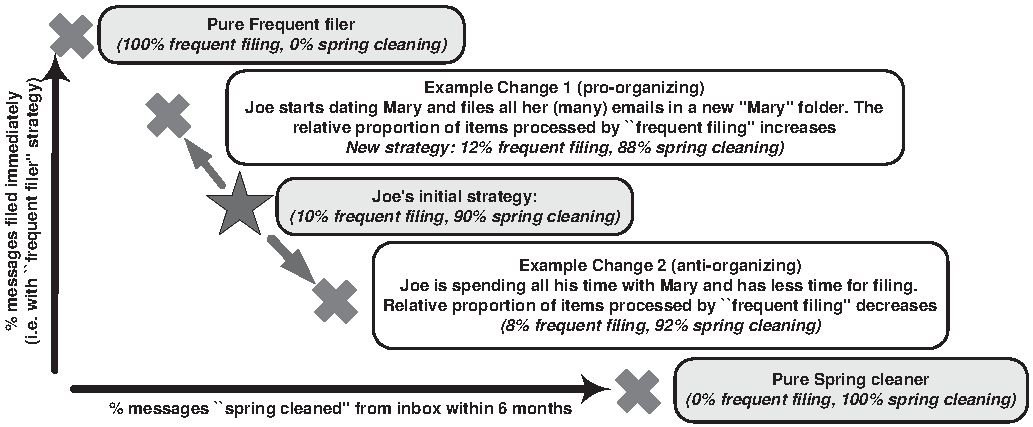
\includegraphics[width=\textwidth]{pictures/discussion/new-change-model.pdf}
	\end{center}
	\caption{A model of changes in email organizing strategy, using the concept of multiple strategies.}
	\label{fig:discussion:new-change-model}
\end{figure}
% CONSIDER: extending model to show both major shifts and minor shifts.}
% ADD: real examples from our study data

%%%%%%%%%%%%%%%%%
% DISCUSS MODEL WHY BIG SHIFTS ARE HARD: 
%%%%%%%%%%%%%%%%%
% Huge amount of work in changing everything.  Easier to change one little thing
% argue in favour of incremental design?
As discussed in \textbf{Section~\ref{discussion:supporting}}, the supporting nature of PIM means that many users devote little time to planning and executing changes in strategy.  Thus it makes sense that only subtle shifts in strategy were observed. As participant M8 commented, there is a huge amount of effort involved in a major reorganization or change in strategy.  Participants noted that such ``grand shifts'' were time-consuming and non-trivial.   Instead, it is much easier to make small adjustments.  Of course, substantial changes in overall trait may occur, but these would happen at major life points and is not unexpected that none were encountered over the course of the study.


%%%%%%%%%%%%%%%%%%%%%%%%%%%%%%%%%%%%%%%%%%%%%%%%
% Use of ``change'' findings in rest of chapter
%%%%%%%%%%%%%%%%%%%%%%%%%%%%%%%%%%%%%%%%%%%%%%%%
% These findings regarding changes are used in a number of ways later in this chapter.
%%%%%%%%%%%%%%%%%%%%%%%%%%%%%%%%%%%%%%%%%%%%%%%%%%%%%%%%%%%%%%%%%%%%%%%%%%%%%
% USE IN EVAL DISC: TO EXPLAIN SUCCESS OF WM, slow change, partial change
%%%%%%%%%%%%%%%%%%%%%%%%%%%%%%%%%%%%%%%%%%%%%%%%%%%%%%%%%%%%%%%%%%%%%%%%%%%%%
The incremental nature of the observed changes in PIM strategy is offered as a partial explanation for the slow/incremental uptake of WM in \textbf{Chapter~\ref{chapter:main-study}}.  Despite the incremental nature of the functionality offered by WM, the change in utilizing mirrored folders is still substantial. The slow rate of changes in PIM strategy may act as an inhibiting factor in the uptake of new tools.  A new tool offering a new form of organization required a huge amount of effort on the part of the user to adopt. Therefore it is envisaged that making folder-mirroring optional is appropriate.

%%%%%%%%%%%%%%%%%%%%%%%%%%%%%%%%%%%%%%%%%%%%%%%%%%%%%%%%%%%%%%%%%%%%%%%%%%%%%%%%%%%%%%%%%%%%%%%%%%%%%%%%%%%%%%%%%
%%%%%%%%%%%%%%%%%%%%%%%%%%%%%%%%%%%%%%%%%%%%%%%%%%%%%%%%%%%%%%%%%%%%%%%%%%%%%%%%%%%%%%%%%%%%%%%%%%%%%%%%%%%%%%%%%
%%%%%%%%%%%%%%%%%%%%%%%%%%%%%%%%%%%%%%%%%%%%%%%%%%%%%%%%%%%%%%%%%%%%%%%%%%%%%%%%%%%%%%%%%%%%%%%%%%%%%%%%%%%%%%%%%
%%%%%%%%%%%%%%%%%%%%%%%%%%%%%%%%%%%%%%%%%%%%%%%%%%%%%%%%%%%%%%%%%%%%%%%%%%%%%%%%%%%%%%%%%%%%%%%%%%%%%%%%%%%%%%%%%

%%%%%%%%%%%%%%%%%%%%%%%%
\subsection{Summary}
%%%%%%%%%%%%%%%%%%%%%%%%

This section has opened up some initial routes for developing an improved conceptualization of PIM strategies -- in terms of cross-tool strategies, and changes over time.

%%%%%%%%%%%%%%%%%%%%%%%%%%%%%%%%
% END: DISCUSSION - CHANGES
%%%%%%%%%%%%%%%%%%%%%%%%%%%%%%%%